\section{DeepDuct: A Deep-Learning Approach to Regional Breast Cancer Classification using Grad-CAM}

\subsection{Accurate Classification of Breast Neoplasms in the BreakHis Dataset}

Transfer-learning the VGG16 on the unmodified BreakHis dataset results in acceptable overall classification accuracy (70\%), however closer inspection reveals bias towards one of the classes (ductal carcinoma) due to imbalances in the number of examples between classes (\emph{Figure \ref{fig:confmat}a}). Oversampling the dataset such that all classes have an equal number of training examples resulted in a small improvement in overall classification accuracy (72\%), and shows a demonstrable reduction in bias (\emph{Figure \ref{fig:confmat}b}).\par

Notably, lobular carcinomas were mistaken for ductal carcinomas in just over two-thirds of the validation set, and correctly identified a quarter of lobular carcinoma examples. Outside the sampling bias, possible explanations for this high false-positive rate include the morphological similarity between the two lesions (lobular carcinomas typically exhibit rounder cells), as well as the low resolution of the dataset, which can degrade visual information of subtle differences. After oversampling the BreakHis dataset, the accuracy and ductal carcinoma false-positive rates have nearly replaced one another, with lobular carcinomas being correctly classified in 63\% of cases and false ductal carcinoma classifications in a quarter of cases. Ductal carcinoma false-positives were in fact halved, on average, across nearly all classes after oversampling.\par

\subsection{Activation Mapping of BreakHis ConvNet using \mbox{Grad-CAM}}

The Grad-CAM algorithm was used to compute class activation maps from the BreakHis fine-tuned VGG16 ConvNet model (\emph{Figure \ref{fig:heatmap}}). In some cases, regions containing artefacts are highly activated and coincide with high-certainty (\textit{i.e.}: high predicted probability) false-positives (\emph{Figure \ref{fig:heatmap}e}). It is also not uncommon for low-certainty false-positives to be activated by similar regions across classes (\emph{Figure \ref{fig:heatmap}f}). Curiously, in many cases correct predictions are made that are largely activated by the stroma, rather than the epithelium (\emph{Figure \ref{fig:heatmap}c}).



\begin{figure}[p]
	\begin{center}
		\caption{Confusion Matrix of VGG16 Model Trained on the Original and Oversampled BreakHis Datasets \label{fig:confmat}}
	\end{center}
	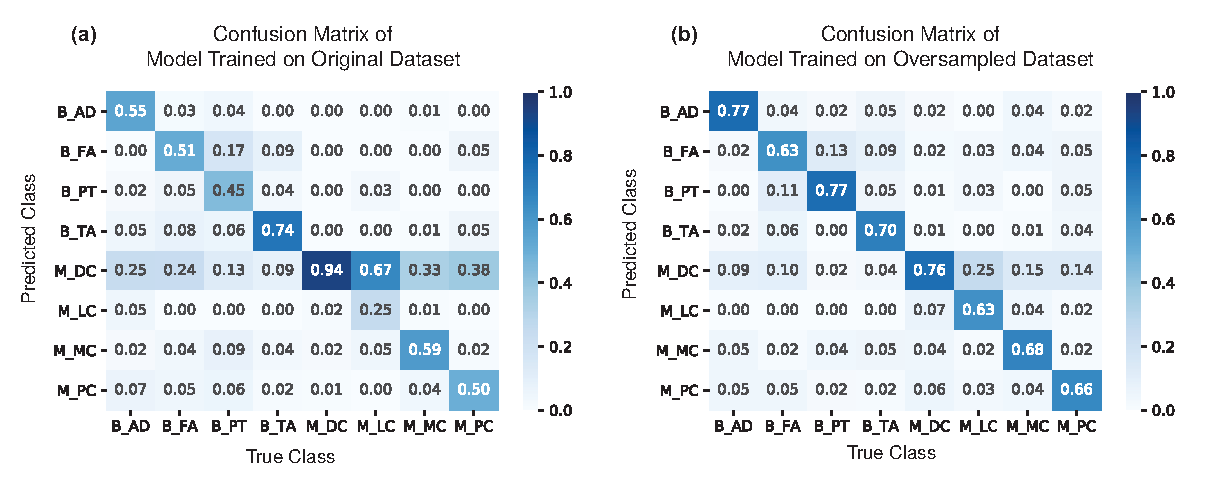
\includegraphics[width=170mm]{figures/deepduct/confusion_matrix.pdf}
	\begin{singlespace}
		\textit{Legend} --- Confusion matrices of the VGG16 model either trained on (a) the original BreakHis dataset as provided by its creators, or (b) a modified version of the BreakHis dataset oversampled such that each class has the same number of training examples. The model trained on the original dataset achieved an average accuracy of 70\% on the validation set across all classes, while the oversampled model saw a modest increase for a final average accuracy of 72\%. See Appendix A for class code legend used in this figure.
	\end{singlespace}
	
\end{figure}

\begin{figure}[t]
	\begin{center}
		\caption{Activation Maps of the BreakHis Fine-Tuned VGG16 ConvNet  \label{fig:heatmap}}
	\end{center}
	\includegraphics[width=150mm]{figures/deepduct/heatmaps.pdf}
	
	
\end{figure}
\begin{figure}[t]
	\begin{singlespace}
		\textit{Legend} --- Selected examples of activation maps of the BreakHis fine-tuned VGG16 model described herein, as calculated by the Grad-CAM algorithm. Column (i) displays the original input image and its ground truth classification. Column (ii) shows the top three predictions of the ConvNet and their activation maps overlayed on the input image; as well as the probability of the classification as reported by the model's softmax layer (shown in brackets). Column (iii) reports the probabilities of the top three predictions in a bar chart. Top probabilities are indicated with a checkmark (\ding{51}) when they match the ground truth (correct classification), and an ``x'' mark (\ding{55}) when they do not (false-positives). Rows (a--c) are examples of correct classifications made by the ConvNet model where the top prediction is of high probability. Rows (d--e) are examples of incorrect classification made by the ConvNet model where the top prediction is of high probability (false-positives). Row (f) is an example of an incorrect classification where none of the classes are reported to be of high-probability.
		
	\end{singlespace}
\end{figure}
